%!TEX root = ../thesis.tex
%*******************************************************************************
%****************************** Third Chapter **********************************
%*******************************************************************************
\chapter{Methodology}
% **************************** Nomenclature **********************************
\nomenclature[u-1-XTrain]{$X_\mathrm{train}$}{Datasets used for training the algorithms}
\nomenclature[u-1-XTest]{$X_\mathrm{test}$}{Datasets used to provide a score for the algorithms}
\nomenclature[u-2-xunknown]{$x_\mathrm{unknown}$}{Data points where the true label is not available to the algorithms used}
\nomenclature[u-2-xknown]{$x_\mathrm{known}$}{Data points where the true label is available to the algorithms used}
\nomenclature[u-3-yunknown]{$y_\mathrm{known}$}{True labels available to the algorithms used}
\nomenclature[u-3-yunknown]{$y_\mathrm{unknown}$}{True labels unavailable to the algorithms used}
% \nomenclature[u-3-ypredict]{$y_\mathrm{predict}$}{Predicted labels by the algorithm}
% **************************** Define Graphics Path **************************

\graphicspath{{Chapter3/Figs/Vector/}{Chapter3/Figs/}}
\section{Outline}
The methodology presents a novel means of assessing different parametrised active learning methods on existing data sets, allowing for a robust answer into the use of active learning in drug rediscovery. Results can thus be given with a given belief. This approach has taken principles commonly used in machine learning and applied it to more traditional algorithmic methods.
\\
Firstly, a collection of pre-existing data sets, $X$, are used. $X$ is then split into two sub sets: $X_{\mathrm{train}}$ and $X_\mathrm{test}$. Similarly to machine learning, the former of these subsets is used in fitting the parameters of the equation, and the latter is used to provide a result without the risk of data leakage into the training set. This is represented in []. Parallelisation is used to efficiently train the algorithms allowing the time for training to be $\sim{}\mathcal{O}(c)$.
\\
Examining the smaller details, each algorithm is provided with the sets $x_\mathrm{known}$, $y_\mathrm{known}$, and $x_\mathrm{unknown}$. Various algorithms are given these sets and allowed to generate a subset of $x_\mathrm{unknown}$ to be added into $x_\mathrm{known}$ alongside corresponding $y_\mathrm{known}$. This can then repeat until a predefined stopping point is reached. Scores are reported using a weighted mean squared error [] based upon $y_\mathrm{predict}$ for all $x$. This is similar to a standard machine learning methodology with a couple of differences. Firstly, no distinction is made between the training and testing set within a dataset contrary to standard practice. This is due to two reasons. Firstly, the datasets are not large enough for an accurate representation of the data within the testing set, and secondly, the scoring to each dataset is not used within the machine learning algorithms to fit parameters as is usually the case. All algorithms used rely upon a simple custom composite model to allow for flexibility and consistency.
\\
In Section [], it was discussed that there are various methodologies of representing chemicals and drugs. ... (if time)
\section{Proof}
In order to demonstrate the effectiveness, a few data sets are used instead, and the program is executed function by function. To start with, the underlying custom functions will be demonstrated, followed by the algorithms and then finally the training framework.

\subsection{Custom Base Functions}
\subsubsection{Split}
The \lstinline{split} function allows for each dataset to be split into $x_\mathrm{known}$, $y_\mathrm{known}$, $x_\mathrm{unknown}$, and $y_\mathrm{unknown}$, as demonstrated in Figure \ref{fig:Split}. This is required as a fundamental step for the algorithmic testing. To demonstrate the validity of this function, ...

\begin{figure}
    \begin{center}
        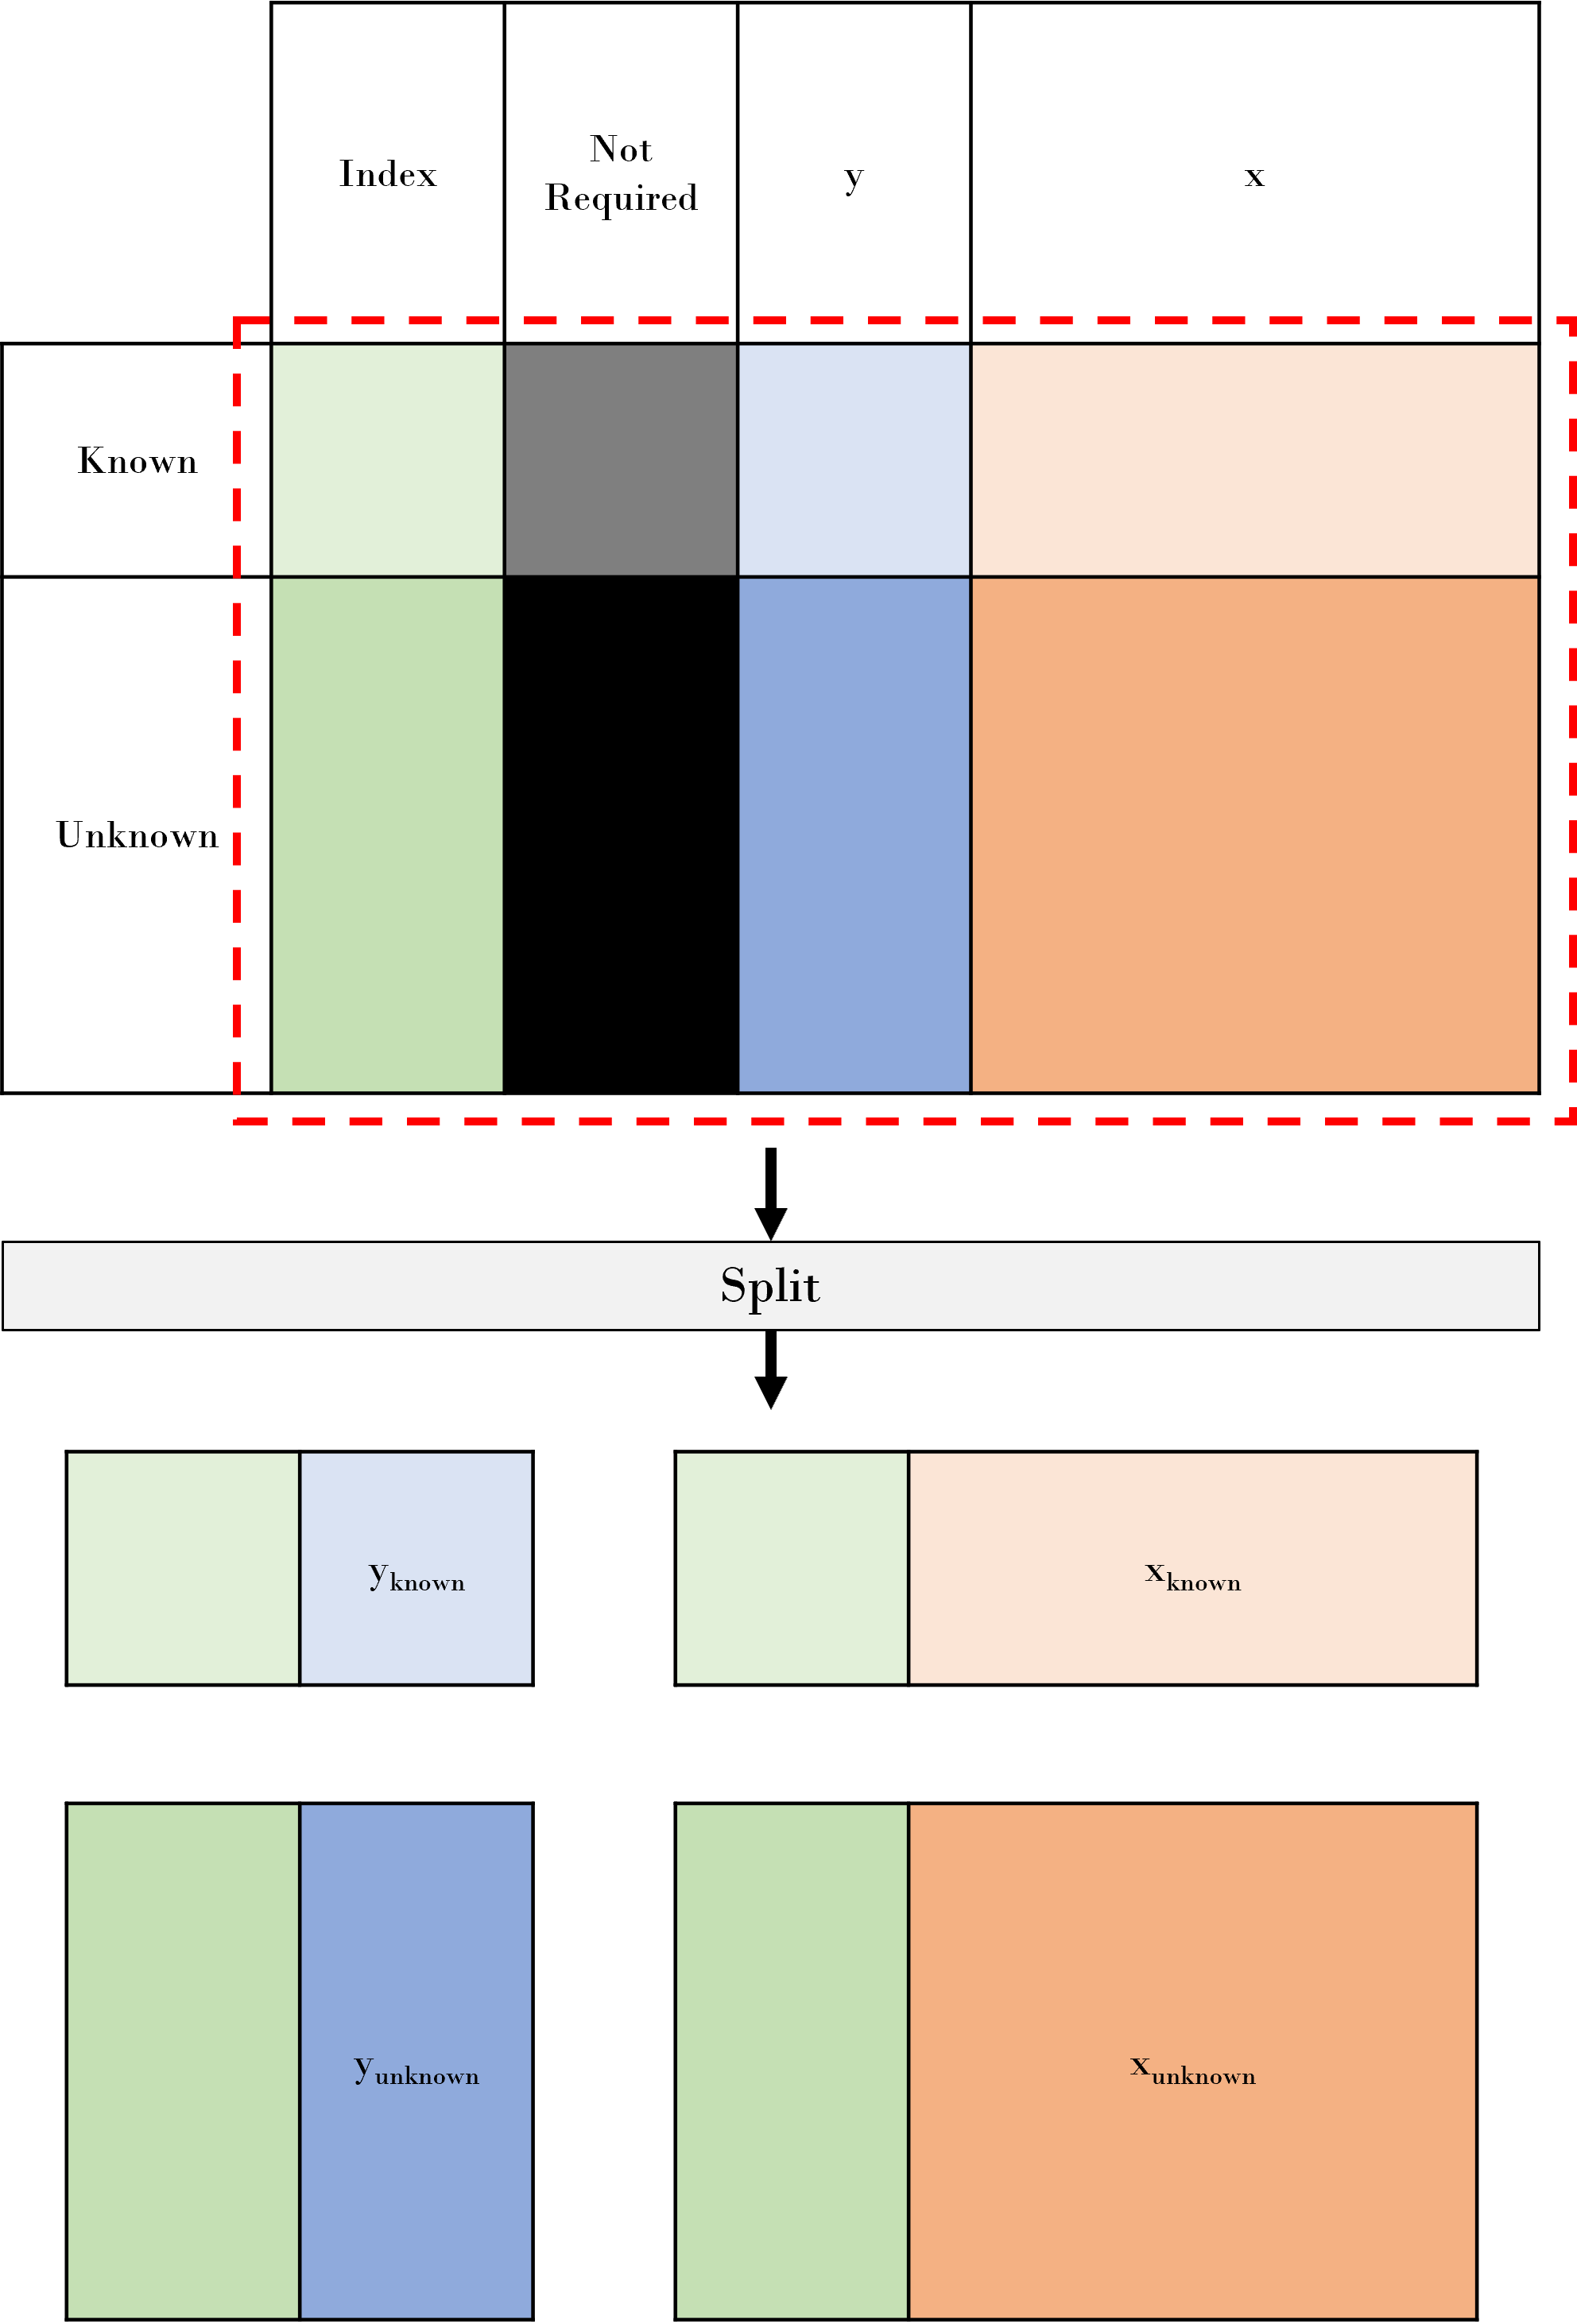
\includegraphics[width=130mm]{split.png}
    \end{center}
    \caption{Graphical representation of the\lstinline{split}function. The red dashed boundary represents the input (additional colour coding has been performed to assist the reader in understanding the transposition of the base components).}
    \label{fig:Split}
\end{figure}


\subsubsection{Repartition}
Upon each iteration, the sets provided to the algorithms need to be repartitioned to allow for the continual operation of the algorithm.
\\
\subsubsection{Model}
\blindtext[1]
\subsubsection{Validate}
\blindtext[1]
\subsection{Active Learning Algorithms}
\blindtext[1]
\subsection{Training Framework}
\blindtext[1]
